\documentclass{sig-alternate}
%\documentclass{article}


\usepackage{enumitem}
\usepackage{framed}
\usepackage{cprotect}
\usepackage{enumitem}
\usepackage{listings}
\usepackage{amstext}
\usepackage{amstext}
\usepackage{pdfpages}
\usepackage{alltt}
\usepackage{epstopdf}
\usepackage{xspace,colortbl}
\usepackage[USenglish]{babel}
\usepackage{multirow}
\usepackage{url}
\usepackage{subfigure}
\usepackage{graphicx}%%
\usepackage{amssymb}
\usepackage{fmtcount}
\usepackage{amsfonts}
\usepackage{xspace}
\usepackage{amsmath}
\usepackage{multirow}
\usepackage[mathscr]{eucal}
%\usepackage{psfrag}
\usepackage{colortbl}

\usepackage{bm}
\usepackage{charter}
\usepackage[nospace]{cite}
\usepackage{csquotes}
\usepackage{enumitem}

\lstset{basicstyle=\large,breaklines=true,language=SQL,belowcaptionskip=.1\baselineskip}

%\linespread{0.975}

\makeatletter
\def\@copyrightspace{\relax}
\makeatother

\begin{document}

%\setlength{\belowdisplayskip}{1pt} \setlength{\belowdisplayshortskip}{1pt}
%\setlength{\abovedisplayskip}{1pt} \setlength{\abovedisplayshortskip}{1pt}
%\setlength{\belowcaptionskip}{-10pt}
%\selectfont

\newtheorem{theorem}{Theorem}
\newtheorem{example}{Example}
\newtheorem{definition}{Definition}
\newtheorem{problem}{Problem}
\newtheorem{property}{Property}
\newtheorem{proposition}{Proposition}
\newtheorem{lemma}{Lemma}
\newtheorem{corollary}{Corollary}

\newcommand{\cond}{\textrm{pred}\xspace}
\newcommand{\dataset}{data set\xspace}
\newcommand{\datasets}{data sets\xspace}
\newcommand{\spview}{\textsf{SPView}\xspace}
\newcommand{\fjview}{\textsf{FJView}\xspace}
\newcommand{\aggview}{\textsf{AggView}\xspace}
\newcommand{\hashfunc}[1]{\textsf{hash}(#1)\xspace}
\newcommand{\hashop}{\textsf{hash}\xspace}
\newcommand{\nsc}{\textsf{NormalizedSC}\xspace}
\newcommand{\rsc}{\textsf{RawSC}\xspace}

\newcommand{\avgfunc}{\ensuremath{\texttt{avg} }\xspace}
\newcommand{\maxfunc}{\ensuremath{\texttt{max} }\xspace}
\newcommand{\minfunc}{\ensuremath{\texttt{min} }\xspace}
\newcommand{\histfunc}{\ensuremath{\texttt{histogram\_numeric} }\xspace}
\newcommand{\countfunc}{\ensuremath{\texttt{count}}\xspace}
\newcommand{\sumfunc}{\ensuremath{\texttt{sum} }\xspace}
\newcommand{\varfunc}{\ensuremath{\texttt{var} }\xspace}
\newcommand{\stdfunc}{\ensuremath{\texttt{std} }\xspace}
\newcommand{\covfunc}{\ensuremath{\texttt{cov} }\xspace}
\newcommand{\corrfunc}{\ensuremath{\texttt{corr} }\xspace}
\newcommand{\medfunc}{\ensuremath{\texttt{median} }\xspace}
\newcommand{\percfunc}{\ensuremath{\texttt{percentile} }\xspace}
\newcommand{\havingfunc}{\ensuremath{\texttt{HAVING} }\xspace}
\newcommand{\selectfunc}{\ensuremath{\texttt{select} }\xspace}
\newcommand{\ratio}{\ensuremath{\rho }\xspace}


\newcommand{\insertion}{\ensuremath{\texttt{INSERT} }\xspace}
\newcommand{\update}{\ensuremath{\texttt{UPDATE} }\xspace}
\newcommand{\delete}{\ensuremath{\texttt{DELETE} }\xspace}

\newcommand{\sysfull}{ActiveClean\xspace}
\newcommand{\sys}{PrivateClean\xspace}
\newcommand{\sysM}{PC\xspace}
\newcommand{\sysnospace}{ActiveClean}

\newcommand{\tbl}[1]{\textsf{#1}\xspace}
\newcommand{\field}[1]{\textsf{#1}\xspace}
\newcommand{\cost}{\textrm{cost}\xspace}
\newcommand{\ans}{\textsf{ans}\xspace}
\newcommand{\dans}{\Delta\textsf{ans}\xspace}
\newcommand{\cqp}{correction query processing\xspace}
\newcommand{\Cqp}{Correction query processing\xspace}

\newcommand{\reminder}[1]{{{\textcolor{magenta}{\{\{\bf #1\}\}}}\xspace}}
\newcommand{\specialcell}[2][c]{%
  \begin{tabular}[#1]{@{}c@{}}#2\end{tabular}}

\def\ojoin{\setbox0=\hbox{$\bowtie$}%
  \rule[-.02ex]{.25em}{.4pt}\llap{\rule[\ht0]{.25em}{.4pt}}}
\def\leftouterjoin{\mathbin{\ojoin\mkern-5.8mu\bowtie}}
\def\rightouterjoin{\mathbin{\bowtie\mkern-5.8mu\ojoin}}
\def\fullouterjoin{\mathbin{\ojoin\mkern-5.8mu\bowtie\mkern-5.8mu\ojoin}}

%\setlength{\belowcaptionskip}{-10pt}

%\newcommand{\reminder}[1] {}
%\pagestyle{plain}

\title{Data Cleaning and Approximate Query Processing on Differentially Private Views}

%\numberofauthors{1}
%\author{\large Sanjay Krishnan, Jiannan Wang, Michael J. Franklin, Ken Goldberg, Tim Kraska{$\,^\dag$} \\
%\vspace{.2em}\affaddr{\large UC Berkeley, ~~ $^\dag$Brown University} \\
%\vspace{.1em}\affaddr{\large \{sanjaykrishnan, jnwang, franklin, goldberg\}@berkeley.edu}\\
%\affaddr{\large tim\_kraska@brown.edu}
%}

%\fontsize{10pt}{12pt}
%\selectfont

%\input{coverletter.tex}

\maketitle

\begin{abstract}
Data are susceptible to various forms of corruption such as missing, incorrect, or inconsistent values.
Almost all of the existing work in data cleaning assumes an interaction model where analysts have unrestricted access to the base data, which is not realistic in many situations concerning personal or sensitive information.
This paper explores a differential privacy mechanism that allows for downstream data cleaning and exploratory analysis.
We propose a framework called \sys which creates private views of a database using a generalization of the well-studied randomized response model.
For large enough datasets, we show thate errors are still detectable even in the private data and can be cleaned. 
We derive finite-sample bounds for estimates of aggregate queries on these cleaned private views.
Our analysis suggests that error is essentially linear in the privacy factor.
\end{abstract}


\section{Introduction}
In 1965, the statistician Stanley Warner noticed that for sensitive questions, survey participation was hampered by the unwillingness of participants to confide in an interviewer \cite{warner1965randomized}.
Consider an auditor exploring the prevalence of bribery in a government office through a survey question: \emph{Yes or No, have you accepted bribe in the last year?}. 
Even with guarantees of anonymity, employees may be reluctant to provide truthful responses.
For such scenarios, Warner proposed the \emph{Randomized Response} model: (1) a participant flips a coin before the interview, (2) if heads, he answers truthfully, and (2) if tails, he selects Yes or No uniformly at random.
Warner showed that such a model provides participants with plausible deniability about their response, yet still allows for rigorous statistical estimation and hypothesis testing.

Since 1965, there have been number of proposals to guarantee privacy while preserving some utility like homeomorphic encryption, value aggregation, and selective censorship \cite{sweeney2002achieving, machanavajjhala2007diversity, li2007t}.
While the aforementioned techniques allow for query answering on private data, they obscure the actual values.
However, raw data rarely starts off in a useful form, and an analyst has to perform a number of preprocessing steps including extraction and resolving inconsistencies prior to query answering--all of which be definition require access to the actual record attribute values.
On the other hand, consider a generalization of Warner's model, where for discrete-valued attributes with probability $p$ replace the value uniformly at random with another value in the domain.   
While any given record can be incorrect, for a large enough dataset, all of the domain values are likely to appear in the the randomized result.
It follows that some types of data cleaning operations, e.g., a find-and-replace, may be possible even on randomized relations (Figure \ref{example}).

However, the challenge is to like Warner's model to meaningful notion of data privacy.
$\epsilon$-differential privacy model~\cite{dwork2011differential} quantifies the privacy of randomized mechanisms.
This is a probabilistic definition of privacy, where $\epsilon$ represents the increase in probability of correctly identifying an individual's response given all other records in a database.
It can be shown that Warner's model is in fact $\epsilon$ differentially private, where $\epsilon$ is inversely related to the randomization probability $p$.
One of the key challenges is selecting meaningful parameter values for the task at hand, i.e., what is the practical difference between $\epsilon = \ln 3$ compared to $\epsilon = \ln 5$~\cite{DBLP:conf/sigmod/YangZMWX12}.

\begin{figure}[t]
\centering
 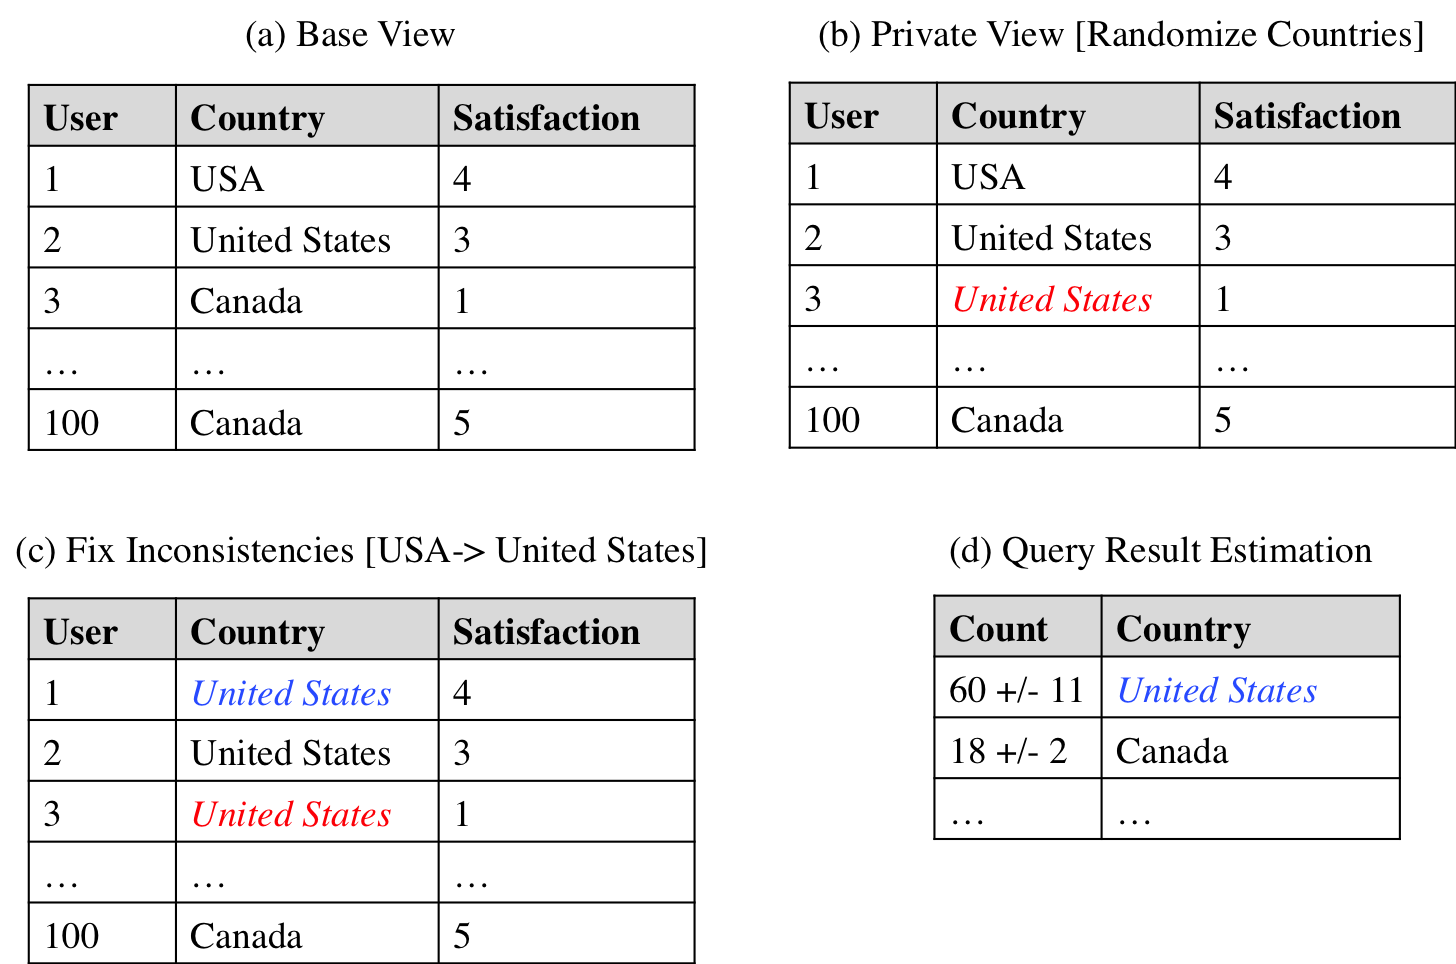
\includegraphics[width=\columnwidth]{figs/example.png}
 \caption{\sys allows users to perform a limited set of cleaning operations on private views of data. Differential privacy preserves attribute domains, and thus, inconsistencies can be identified in even provably private views.\label{example}}\vspace{-2em}
\end{figure}

In this paper, we present \sys a framework for data cleaning and approximate query processing on differentially private relations.
We assume that there is a trusted curator of a database $D$, and an untrusted analyst who wishes to analyze a view of this database $V$ which consists of numerical (integer or real valued) attributes and possible dirty discrete valued attributes.
We apply a generalized version of Warner's randomized response technique called, Generalized Randomized Response (GRR), to the view $V$.
This view is provably private for any desired level of privacy $\epsilon$.
Analysts can apply a restricted set of deterministic data cleaning operations to clean the dirty discrete attributes.
Then, we provide an estimation framework to estimate the result of \sumfunc, \countfunc, and \avgfunc queries on the cleaned private relation.
The system is self-tuning and can select a level of privacy to ensure that any dirtiness in the discrete attributes can be detected with probability of at least $1-\alpha$ or that all subsequent aggregate queries are guaranteed to be within $\delta\%$ accuracy with high probability.

There are a number of technical contributions in this paper.
First, we formalize the class of data cleaning operations that can be supported on a GRR view, and we model the effects of data cleaning as a bi-partite graph mapping dirty values to cleaned values.
We can use this graph to estimate false positive values included in aggregate queries with predicates. 
Next, we analyze the system statistically both in the finite-sample case and in the asymptotic case to understand the tradeoff between privacy, cleanability, and query accuracy.
Finally, we show how this analysis can be inverted to select maximal privacy levels given some constraint on query accuracy or cleanability.
















\section{Background}
Before introducing \sys, we will provide context to the problem.

\subsection{Motivating Example}
To understand how we can have non-trivial privacy constraints but still allow for data cleaning, consider the following scenario.
We are using an online application to collect course evaluations (e.g. M-CAFE \cite{zhou2015m}).In a simplified model, the data are collected in a relation $R$ with a categorical \textsf{major} attribute and one numerical \textsf{score} for the instructor (0-100):
\[
R(score,major)
\] 
Even though the data are anonymous, the relation $R$ is not private.
The instructor might be able to identify individuals with rare \textsf{major} values, and consequently, may penalize those who left a low score.

Now suppose we want to release the relation $R$ for analysis by the course instructors.
Let $M$ be the set of all majors, we can apply the following privacy mechanism: with probability $p$ replaces $r[score]$ with a random value from $M$. 
Intuitively, if the relation is large enough (we will formalize this precisely later), it is likely that by chance those rare demographics will be assigned to at least a few other students; affording some level of ambiguity.
From a data cleaning perspective, even though the individual records have been randomized, the domain is still preserved.
Errors that do not require record-level information can still be cleaned. 
For example, suppose \textsf{major} has alternative representations of the same logical value ``Electrical Engineering and Computer Sciences" and ``EECS".

It turns out that this is a little bit of an over-simplification, and to answer queries will require re-weighting results appropriately to account for the cleaning.
Furthermore, we will also have to apply randomization to the \textsf{score} attribute.
Consider the case when there is a very strong correlation between \textsf{major} and \textsf{score}, e.g., all Civil Engineering majors gave a \textsf{score} of 1. 
This can de-privatize our results, and we will discuss the solution to this problem in subsequent sections.
However, in this section, for ease of presentation, we will use this simplified model as a running example.

\subsection{Local Differential Privacy}
Local differential privacy is a measure of randomness in record-by-record transformations.
There is a parameter $\epsilon$, where larger values implies less randomness.
Let $R$ be a relation over the attributes $A$. A randomized algorithm
$M:R\mapsto\mathcal{D}$ is said to be $\epsilon$-local differentially
private if for all records $r,r'\in R$ and for any measurable subset
$S$ of the range of $M$:
\[
\sup_{r,r'}\frac{P[M(r)\in S\mid r]}{P[M(r')\in S\mid r']}\le\exp(\epsilon)
\]
In other words, given some observed randomized result $S$, $\epsilon$ is a bound on the ratio between the most likely input and the least likely input.

\noindent\textbf{Example of $\epsilon=0$: } This implies perfect privacy where observation of the private output does not make any input any more likely. An example of this would be an ideal one-way hash function.

\vspace{0.5em}

\noindent\textbf{Example of $\epsilon=\infty$: } Note that this does not imply no privacy. This only implies that observation of the private output excludes certain inputs. An example of this would be adding uniform random noise in $[-1,1]$ to numerical attributes. 

\begin{example}
Suppose a record $r$ from the course evaluation dataset has a \textsf{major} of ``Civil Engineering".
After applying the randomization, with probability $\approx 1-p$\footnote{The probability is not quite $1-p$, it is $1-p+p\frac{1}{N}$} the value stays the same ``Civil Engineering", else it is set to another value.
Due to symmetry $\epsilon = \ln \frac{1-p}{p}$.
\end{example}

\subsection{Database Model and Assumptions}
We formalize the intuition from the course evaluation example.
Let $R$ be a relation of a set of numerical attributes $A = \{a_1,...,a_k\}$, and a set of discrete valued attributes $D = \{d_1,...,d_l\}$.
We explore aggregate queries $f$ on this relation of the following form:
\begin{alltt}
SELECT \textsf{f}(a) FROM R WHERE cond(d)
\end{alltt}
where $a$ is a numerical attribute, and $d$ is a discrete attribute.

We consider data corruption in the discrete attributes of $R$.
In particular, there is a clean relation $R_{clean}$ (with the same schema as $R$) in which records have a one-to-one mapping with the dirty records.
This does not include record duplication errors or other types of schema errors.
We assume that these errors can be fixed using \emph{local} data cleaning operations (formalized subsequently).

\subsection{Local Cleaners}
We assume the existence of deterministic local data cleaning operations.
Let the set of discrete attributes $D$ be partitioned into $k$ subsets denoted by $g_i$:
\[
D = \cup_i^k g_i
\] 
Each \emph{local} cleaner $C_i(\cdot)$ is associated with a $g_i$, that is, given a record projected along $g_i$ it deterministically cleans the projection:
\[
g_i \subseteq D \text{ , } C_i : R[g_i] \mapsto R_{clean}[g_i]
\]
In other words, these cleaners can repair a discrete value only given local information, i.e., a subset of other attributes.
The cardinally of $g_i$ has implications on the granularity of privacy that is possible.
This is a restrictive assumption, but there are a number of common settings where such cleaners exist.

\begin{example}
Suppose \textsf{major} has alternative representations of the same logical value ``Electrical Engineering and Computer Sciences" and ``EECS". The find-and-replace operation ``Electrical Engineering and Computer Sciences -> EECS" is a local cleaner along the \textsf{major} attribute.
\end{example}

\begin{example}
Consider \textsf{major} values of ``Electrical Engineering and Computer Sciences" and ``Civil Engineering". The extract operation that finds the phrase ``Engineering" is a local cleaner along the \textsf{major} attribute.
\end{example}

\begin{example}
Suppose one student had \textsf{major} value of ``NULL". The value filling operation is \textbf{NOT} a local cleaner since it cannot be fixed given the information in the relation.
\end{example}

\begin{figure}[t]
\centering
 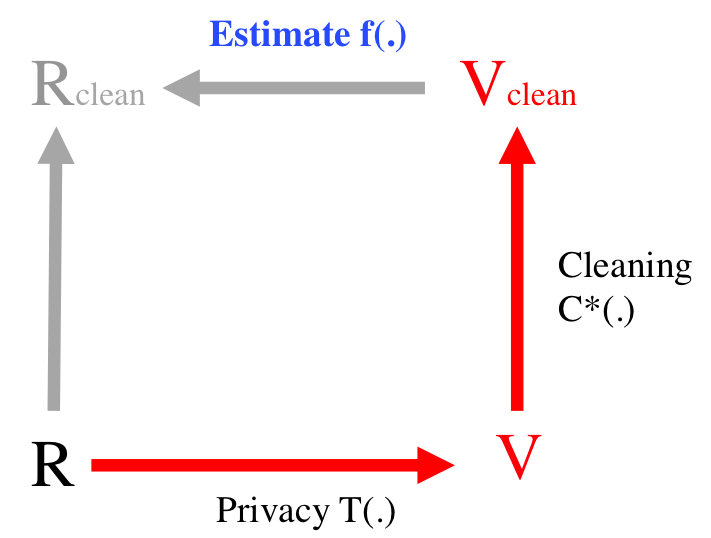
\includegraphics[width=0.6\columnwidth]{figs/example2.png}
 \caption{We want to give users the ability to query the private cleaned view while estimating the result if the query and the data cleaning were applied to original relation. \label{example2}}
\end{figure}

\subsection{Goals of \sys}
Figure \ref{example2} illustrates the primary goal of this work.
A trusted curator applies a randomized transformation $T(\cdot)$ to a dirty relation $R$.
We assume that while the local cleaners are not known to the curator, she does know the partition over discrete attribute values $\{g_1,...,g_k\}$.
The result is a private view $V$.
The untrusted user applies local cleaners to $V$ resulting in $V_{clean}$.
Given an aggregate query $f$ and $V_{clean}$, the goal is to estimate the result of $f(R_{clean})$.
Of course, since the privacy is randomized this estimate is a random variable.
The goal of this work is to present an initial set of analyses about variance and the possibility of the estimate (ultimately related to accuracy).

\noindent We present analysis about the following properties:

\vspace{0.5em}

\noindent\textbf{$\alpha$-error detectability: } Let $r[d]$ be a dirty attribute value, then with probability $1-\alpha$ there exists a record $v \in V$ with the value $r[d]$. Intuitively, this means that an error can be detected with failure rate $\alpha$ over all possible randomized instances of the private view.

\vspace{0.5em}

\noindent\textbf{Unbiasedness: } Let $\hat{q}$ ~ be an estimate of $f(R_{clean})$ based on $V_{clean}$. Unbiasedness means that the expectation of $\mathbf{E}[\hat{q}]$ over all possible randomizations is the true value $f(R_{clean})$.

\vspace{0.5em}

\noindent\textbf{$\alpha$ confidence interval: } Let $\hat{q}$ be an estimate of $f(R_{clean})$. We want a confidence interval of $\pm \delta$ with probability $1-\alpha$. This represents the probability that the estimate deviates from the true value by more than $\delta$.

\begin{example}
A user receives a private view $V$ of the course evaluations, and she wants to count the number of engineering students that responded to the survey.  
She applies an extract operation that finds the phrase ``Engineering" in the \textsf{major} attribute, and runs the SQL query.
\sys estimates the number of engineering students in the original relation.
\end{example}


\section{Architecture and \\Problem Formalization}
In this section, we formalize the technical challenges addressed in this work.

\subsection{Problem 1. Cleanable Private Views}
The first problem that we address is to develop a $\epsilon$-local differentially private mechanism that allows for local cleaning.
Given a dirty relation $R$, the set of numerical attributes $A$, discrete attributes $D$, and a partition set of the discrete attributes $G$, \textbf{find a $\epsilon$-local differentially private transformation $T(\cdot)$ such that errors can be detected in $V=T(R)$ with an probability of $1-\alpha$ for any $\alpha \in (0,1)$.}

In our motivation, we alluded that the solution to this problem is a multi-column generalization of Warner's randomized response model.
However, there are few new issues, practical and theoretical, that we will subsequently address.
First, what is the dependence on the dataset size, and how many records are needed before the mechanism provides meaningful results.
Next, how do we ensure that randomization preserves enough structure such that the cleaners can still be used, i.e., preserve the domain of $g_i$.
Finally, how should we handle the numerical attributes.

\subsection{Problem 2. Cleaning and Aggregates}
The next problem that we explore is data cleaning and aggregate query result estimation on cleaned private views of data.
Let $V$ be a private relation and let $V_{clean}$ be a cleaned private relation after applying local cleaners.
For a \sumfunc, \countfunc, \avgfunc aggregate query $f$ with predicates, \textbf{estimate the result of the aggregate query $f$ with confidence intervals.}

The PrivateClean problem describes query processing on cleaned private relations. 
It turns out that the data cleaning operations change the statistical properties of the
randomization and these will have to be incorporated into the estimates.
Furthermore, we analyze two theoretical problem settings the asymptotic case and the finite sample case.

\subsection{Architecture}
Figure \ref{architecture} describes the architecture of \sys.
The system is initialized with a view of a database $R$, and \sys applies a randomized transformation and releases the private view.
\sys provides an API that allows for users to estimate aggregate query results using the private data after a restricted number of data cleaning operations.
The estimator manages the provenance of rows in the cleaned private view to correspond them with rows prior to cleaning.

\begin{figure}[t]
\centering
 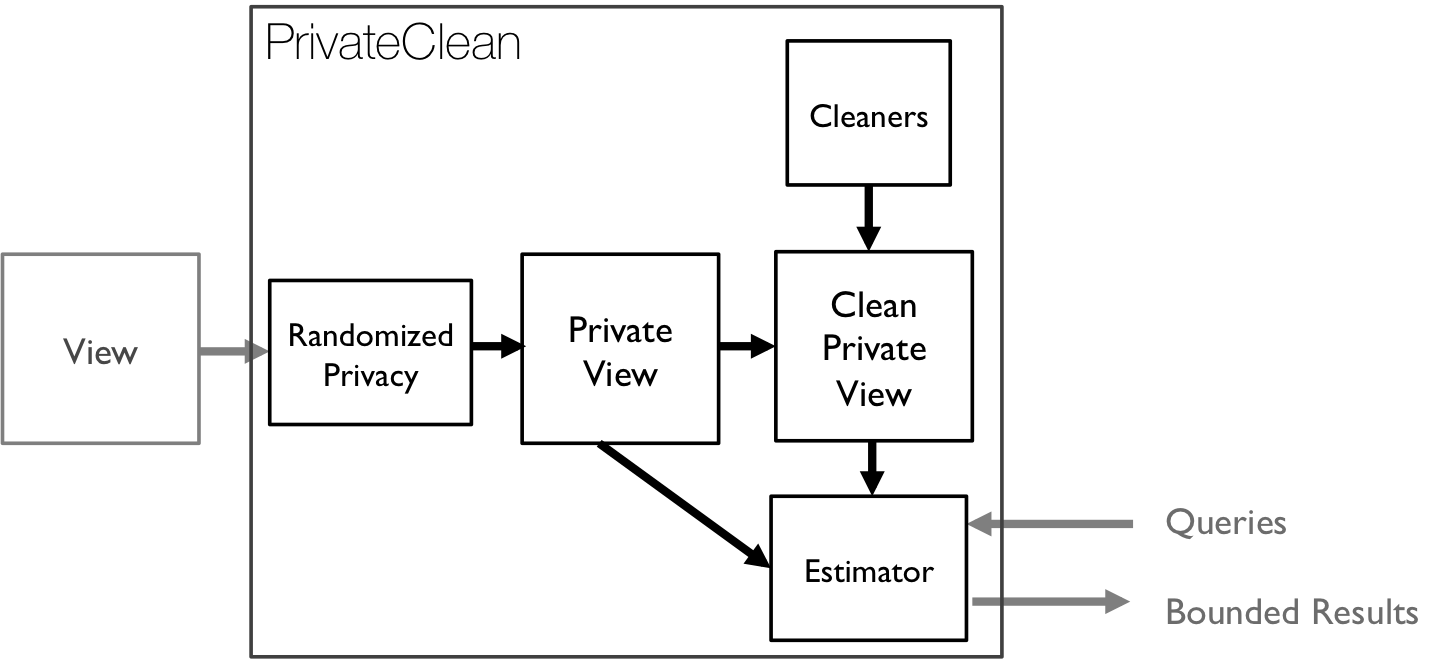
\includegraphics[width=\columnwidth]{figs/architecture.png}
 \caption{The architecture of \sys \label{architecture}}
\end{figure}

\section{Generalized Randomized \\ Response (GRR)}
This section presents our solution to Problem 1 by designing a privacy mechanism that allows for some types of data cleaning.

\subsection{Discrete Attributes}
Let $g_i$ be a partition of the discrete attribute set.
Each $g_i$ defines a n-tuple of attributes of $R$.
Let $Domain(g_i)$ be the set of all the distinct tuple values in $R[g_i]$.
Then, for each $g_i$, we apply a randomized response mechanism:
\[
r'[g_i] = \begin{cases} r[g_i] & \text{w.p } 1-p_i \\ 
\mathbf{U}(Domain(g_i)) & \text{w.p } p_i \end{cases}
\]
where $\mathbf{U}(\cdot)$ selects an element uniformly at random. 

\begin{lemma}[Randomized Response Mechanism]
With the random replacement mechanism, the projection of each categorical attribute $\Pi(g_i)$ is $\epsilon$-local differentially private, with $\epsilon = \ln (\frac{3}{p_i} - 2)$. 
\end{lemma}

\iffalse
\begin{proof}
Let $N = \mid Domain(g_i) \mid$:
\[
\epsilon = \ln \frac{1-p_i + p_i \frac{1}{N}}{p_i \frac{N-1}{N}}
\] 
The worst case is when there are only two values in the domain and all of the other entries in the database are one value except for one, then this gives us $N=2$, plugging it in to the above formula:
\[\epsilon = \ln (\frac{3}{p_i} - 2)\]
\end{proof}
\fi

\subsection{Numerical Attributes}
We discussed the subtle de-randomization problem with numerical attributes in the previous section.
We have to randomize the numerical attributes as well.
However, in general, with numerical attributes $N = \mid R \mid$ making the randomized response model not meaningful.
For such attributes, instead we use the following mechanism.
For each numerical attribute $a_i$, 
\[
r'[a_i] = \mathbf{L}(r[a_i],b_i)
\]
Where $\mathbf{L}(\mu,b)$ is the Laplace distribution:
\[
\mathbf{L}(\mu,b) \sim \frac{1}{2b}\exp (\frac{\mid x - \mu\mid}{b})
\]

\begin{lemma}[Laplace Mechanism]
The Laplace Mechanism is $\epsilon$-local differentially
private, with $\epsilon = \frac{\Delta_i}{b_i}$. Where $\Delta_i$ is defined as the max
difference between any two values in $\Pi(a_i)$.
\end{lemma}

\subsection{GRR Summary}
To summarize, the GRR mechanism takes as input a set of numerical attributes $A$ and a set of partitioned discrete attributes $G$.
For each partition $g_i$ there is a user-specified privacy parameter $p_i$ which is its randomization probability, and for each numerical attribute $a_i$ there is a parameter $b_i$ which is the amount of Laplace noise to add.
For each numerical attribute, we apply the Laplace mechanism with $b_i$, and for each discrete attribute partition, we apply randomized response with probability $p_i$. 
Using the composition lemma from Dwork et al., we prove the following result about the GRR Clean Mechanism:

\begin{theorem}[Generalized Randomized Response]
For a set of numerical and discrete attributes. The Generalized Randomized Response is an $\epsilon$ locally differentially private mechanism with $\epsilon = \sum_{n_i} \epsilon_{n_i} + \sum_{g_i} \epsilon_{g_i}$, where $\epsilon_a$ is appropriate calculated using the lemmas above.
\end{theorem}

\begin{example}
For course evaluation example, suppose $p_0$ is probability $0.25$, and $b_0 = 50$.
For the discrete attribute value $\epsilon = 2.3$ and for the numerical attribute $\epsilon=2$.
The total privacy is $\epsilon = 4.3$.  
\end{example}

\subsection{Analysis}
The efficacy of the GRR model for data cleaning relies on a property we call $\alpha$-error detectability which we formalized earlier.
Due to randomization there is some probability that an error that affects one record will be masked, and we want to know how large the dataset needs to be before with high probability ($1-\alpha$) the erroneous value is seen even in the GRR view. 
The corollary to this analysis is that $\alpha$ allows us to intuitively select $p_i$ and $b_i$ such that errors are detectable. 

We first consider a lemma about the domain of a single discrete attribute partition $g_i$:
\begin{lemma}
For an attribute $g_i$, and a dataset size $S>\frac{N}{1-p_i}\ln(\frac{1}{\alpha})$, with probability $1-\alpha$ the domain is preserved. 
\end{lemma}
\iffalse
\begin{proof}
First, let us start with the
probability that one value $x$ is not preserved:
\[
P[x\text{ is masked}]=\alpha=[\frac{p(N-1)}{N}]^{S}
\]
If we solve for $S$, apply the inequalities that $\frac{N-1}{N}\le1$
and $ln(x)\le x-1$, we get
\[
\frac{\ln(\frac{1}{\alpha})}{1-p}\le S
\]
Then applying a union bound we get:
\[
\frac{N}{1-p}\ln(\frac{1}{\alpha})\le S
\]
\end{proof}
\fi
The lemma shows that increased privacy, namely increasing $p_i$, requires a larger dataset to ensure that all attribute values are seen in the GRR view.
What is interesting is that this probability is linear in $\frac{1}{1-p}$ and the number of distinct values in the domain.

We can apply a union bound over all of the attribute partitions:
\begin{theorem}
A dataset size of $S$ greater than:
\[
S\ge(\sum_{i}\frac{N_{i}}{1-p_{i}})\ln(\frac{1}{\alpha})
\]
ensures $\alpha$-error detectability.
\end{theorem}
\iffalse
\begin{proof}
We apply a union bound to arrive at the formula:
\[
S\ge(\sum_{i}\frac{N_{i}}{1-p_{i}})\ln(\frac{1}{\alpha})
\]
\end{proof}
\fi

\begin{example}
For the course evaluation example, let us suppose $p_i$ is 0.25 and there are 25 distinct majors in the dirty relation. To have 95\% error detectability, we need approximately 100 records, and for 99\%, we need 154 records.
\end{example}

\subsection{Privacy Tuning}
We can use the expression for $S$ to tune the privacy parameters $p$ and $b$. 
In particular, can find the max $p$ for $1-\alpha$-error detectability.
Then, we can set each $b_i$ such that each of the projections is at least as private the other attributes.

%We can use this analysis to determine the maximum value of $p$ that allows for $\alpha$ error detectability:
\begin{corollary}
For a desired domain preservation probability $1-\alpha$, dataset size $S$,
the maximum randomized response privacy parameter is $p_{max}=1-\frac{(1-\alpha)\sum_{i}N_{i}}{S}$.
\end{corollary}
\iffalse
\begin{proof}
\[
\frac{\sum_{i}N}{1-p_{max}}\ln(\frac{1}{\alpha})\ge(\sum_{i}\frac{N_{i}}{1-p_{i}})\ln(\frac{1}{\alpha})
\]
\[
\frac{\sum_{i}N}{1-p_{max}}\ln(\frac{1}{\alpha})=S
\]
\[
\frac{1}{1-p_{max}}=\frac{S}{\ln(\frac{1}{\alpha})\sum_{i}N_i}
\]
\[
p_{max}\ge1-(1-\alpha)\frac{\sum_{i}N_i}{S}
\]
\end{proof}
\fi

Using this analysis, we can arrive at the following tuning algorithm which ensures $1-\alpha$ error detectability and uniform privacy with the numerical attributes:
\begin{enumerate}
\item \textsf{Input: } Error detectability parameter $\alpha$.
\item \textsf{Output: } For each $g_i \in G$ find $p_i$ and for each $a_i \in A$ find $b_i$.
\item For each $g_i \in G$, find the number of distinct values $N_i$.
\item Set all $p_i$ to $p = 1-(1-\alpha)\frac{\sum_{i}N_i}{S}$.
\item For each $a_i \in A$, let $\min i$ be the minimum value and $\max i$ be the maximum value.
\item Set all $b_i = \frac{(\min i - \max i)}{\ln (\frac{3}{p} - 2)}$ 
\end{enumerate}

In the rest of the paper, we will assume that $p_i$ and $b_i$ are given, either set by the tuning algorithm or user-specified.
Furthermore, we will assume that the dataset is sufficiently larger to ensure $\alpha$-error detectability.




%\section{$\alpha$ Error Detectability}
We first present analysis about the privacy mechanism itself, and how successfully an analyst can detect errors in a private relation.



To analyze this, we first consider a lemma about the domain of a single attribute group:
\begin{lemma}
For a dataset size $S>\frac{N}{1-p}\ln(\frac{1}{\alpha})$, with probability
$1-\alpha$ the domain is preserved. First, let us start with the
probability that one value $x$ is not preserved:
\[
P[x\text{ is masked}]=\alpha=[\frac{p(N-1)}{N}]^{S}
\]
\end{lemma}
\begin{proof}
If we solve for $S$, apply the inequalities that $\frac{N-1}{N}\le1$
and $ln(x)\le x-1$, we get
\[
\frac{\ln(\frac{1}{\alpha})}{1-p}\le S
\]
Then applying a union bound we get:
\[
\frac{N}{1-p}\ln(\frac{1}{\alpha})\le S
\]
\end{proof}

Applying a union bound over the lemma we get:
\begin{theorem}
A dataset size of $S$ greater than:
\[
S\ge(\sum_{i}\frac{N_{i}}{1-p_{i}})\ln(\frac{1}{\alpha})
\]
ensures $\alpha$-error detectability.
\end{theorem}
\begin{proof}
We apply a union bound to arrive at the formula:
\[
S\ge(\sum_{i}\frac{N_{i}}{1-p_{i}})\ln(\frac{1}{\alpha})
\]
\end{proof}

We can use this analysis to determine the maximum value of $p$ that allows for $\alpha$ error detectability:
\begin{corollary}
For a desired domain preservation probability $1-\alpha$, dataset size $S$,
the maximum randomized response privacy parameter is $p_{max}=1-\frac{(1-\alpha)\sum_{i}N_{i}}{S}$.
\end{corollary}
\begin{proof}
\[
\frac{\sum_{i}N}{1-p_{max}}\ln(\frac{1}{\alpha})\ge(\sum_{i}\frac{N_{i}}{1-p_{i}})\ln(\frac{1}{\alpha})
\]
\[
\frac{\sum_{i}N}{1-p_{max}}\ln(\frac{1}{\alpha})=S
\]
\[
\frac{1}{1-p_{max}}=\frac{S}{\ln(\frac{1}{\alpha})\sum_{i}N}
\]
\[
p_{max}\ge1-(1-\alpha)\frac{\sum_{i}N}{S}
\]
\end{proof}

\section{Data Cleaning on GRR Views}
The first part of our solution to Problem 2 relates to modeling the data cleaning.
We describe how data cleaning affects the statistics of queries on a GRR view.
To do so, we will have to keep track of provenance, i.e.,  the mapping between original values before data cleaning and the values after cleaning.
Since the predicates of our queries apply to single discrete attributes, and our data cleaning is applied to the partitioned groups $g_i$, without loss of generality, we present this section for only a single partitioned group $g_i$.

\subsection{Value Provenance Graph}
The local cleaning model defines a directed bipartite graph over distinct values.
Let $L$ be the set of distinct values of the GRR view before data cleaning, and let $M$ be the set of distinct values after data cleaning. Each $l \in L$ and each $m \in M$ defines a node in the bipartite graph. 
We add edges between $L$ and $M$ to represent the transformation made by a local cleaner.
However, even with deterministic local cleaners, there might be a many-to-one mapping.
It turns out that the deterministic local cleaner definition disallows one-to-many mappings, and we will exploit this structure for query result estimation.
An example of a \emph{one-to-many} local cleaner is one that with probability $0.5$ assigns one value or assigns another; a model which while theoretically possible is uncommon.

\begin{lemma}
Let $g_i$ be an discrete attribute partition, and $C_i$ be a local cleaner. The directed bipartite graph generated from $V$ and $V_{clean}$ is \textbf{fork-free}, that is there are no one-to-many mappings.
\end{lemma}

\begin{figure}[t]
\centering
 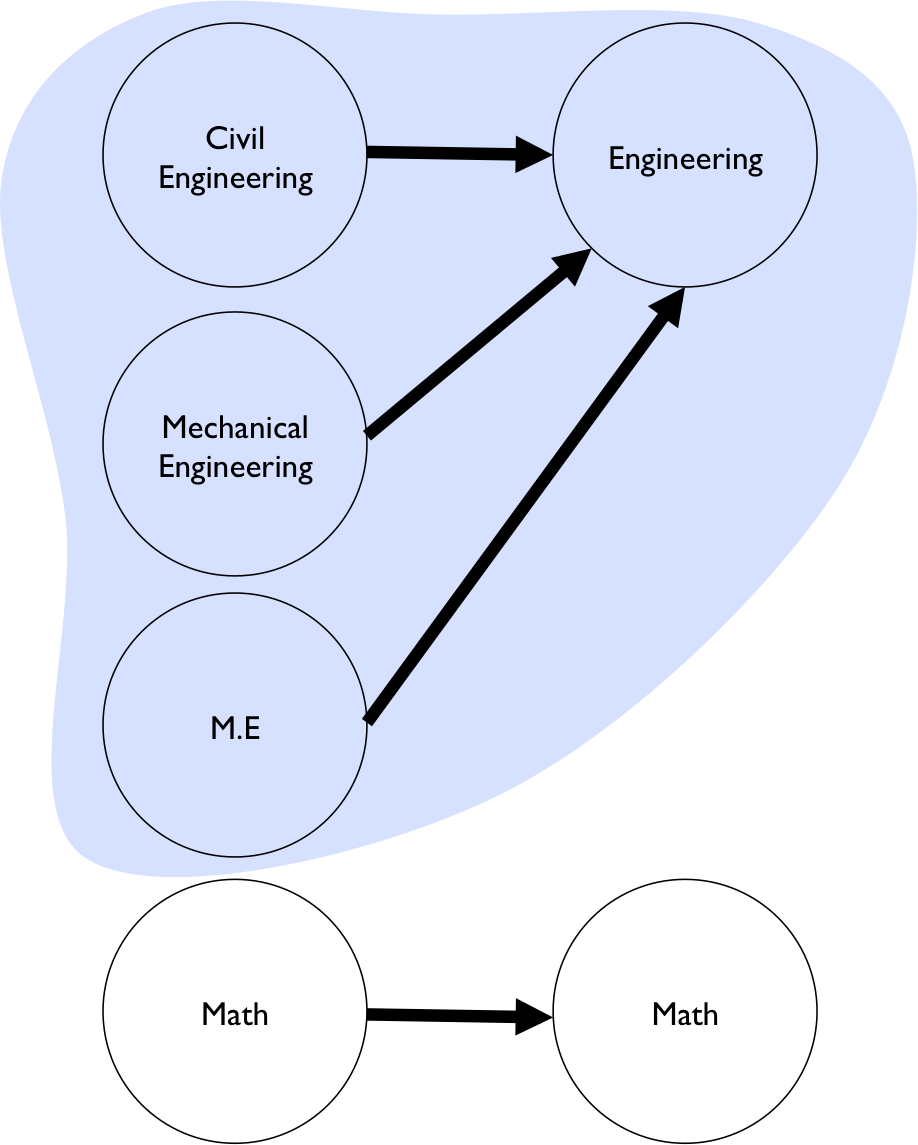
\includegraphics[width=0.5\columnwidth]{figs/graph.png}
 \caption{Local data cleaning operations can be described as a bipartite graph mapping old values to new ones. Predicates on cleaned relations can be interpreted as vertex cuts on the clean partition of the graph.\label{architecture}}
\end{figure}

\subsection{Predicates As Vertex Cuts}
Intuitively, the goal is for any predicate, which can be thought of as a subset of $M$, to quantify the false positive rate (records falsely included) and false negative rate (records falsely excluded) due to the randomization. 
This graph gives us a convenient abstraction to essentially count the number of edges affected by a predicate.
We consider predicates over a single attribute $d_i$.
Let $cond(d_i)$ be a predicate and each predicate can be expressed as a subset $M_{pred} \subseteq M$.
Each $L_{pred}$ will have a parent set $L_{pred}$, that is the set of vertices in $L$ with an edge to exactly one $m \in M_{pred}$.
Together $cut = (L_{pred},M_{pred})$ defines a cut on the bipartite graph.

\begin{example}
Suppose we have a dirty \textsf{major} of four values ``Civil Engineering", ``Mechanical Engineering", ``M.E", ``Math".
The local cleaner maps the first three values to ``Engineering", and the user's predicate queries ``Engineering".
$L_{pred}$ is the set that contains ``Civil Engineering", ``Mechanical Engineering", ``M.E".
$M_{pred}$ is singleton set with ``Engineering".
\end{example}

\begin{example}
Now let us consider an example with multiple attributes in $g_i$, and suppose $g_i$ was (\textsf{city}, \textsf{state}). 
The view has ``San Francisco, CA", ``San Francisco, NULL", ``New York, NY".
The local cleaner maps ``San Francisco, NULL" to ``San Francisco, CA", and if the user's predicate queries the \textsf{state} ``CA", then $L_{pred}$ is ``San Francisco, CA", ``San Francisco, NULL", and $M_{pred}$ is the singleton with ``San Francisco, CA".
\end{example}

\subsection{Predicate Probability Estimation}
When the user issues an aggregate query to a GRR view, there will be a false positive (records falsely included) and false negative rate (records falsely excluded).
Using this graph, we can estimate the false positive and false negative rates of a predicate.
Let $r \in R$ be a row from the original non-private relation.
Let $r' \in R_{clean}$ be a row from the hypothetical cleaned non-private relation.
Making the assumption from the section that the dataset is large enough such that the entire domain is visible in the GRR view and the fork-free nature of the bipartite graph, it is easy verify the following lemma:
\begin{lemma}\label{pre-image}
For an attribute $d_i \in g_i$, if and only if $cond(r'[d_i])$ is true then $r[d_i] \in L_{pred}$.
\end{lemma} 

Following from this lemma, to quantify the false positive and false negative rates of the predicate, we need to estimate the probability that after randomization a record is falsely in $L_{pred}$ or falsely excluded from $L_{pred}$ respectively.
Let $l = \mid L_{pred} \mid$, and $r[d_i] \in L_{pred}$.
The true positive probability is: 
\[
\tau_p = (1-p) + p \frac{l}{N}
\]
The false positive probability is: 
\[
\tau_n = p \frac{l}{N}
\]
Likewise, suppose $r[d_i] \not\in L_{pred}$, the true negative probability is:
\[
\gamma_p = (1-p) + p \frac{N-l}{N}
\]
and the false negative probability is:
\[
\gamma_n = p \frac{N-l}{N}
\]

From a statistical estimation perspective $p$ and $l$ are deterministic values known to the query processing system.
Therefore, $\tau_p,\tau_n,\gamma_p,\gamma_n$ are deterministic values.
In the following section, we show that this determinism allows for unbiased estimates of the aggregate queries.

\subsection{Note About Assumptions}
In proving Lemma \ref{pre-image}, we apply two assumptions: the dataset is large enough such that the entire domain is visible in the GRR view and the fork-free nature of the bipartite graph.
This lemma is instrumental in calculating deterministic values for $\tau_p,\tau_n,\gamma_p,\gamma_n$.
However, without these assumptions it is significantly harder to estimate $\tau_p,\tau_n,\gamma_p,\gamma_n$, since the lemma is no longer true.
If the entire domain is not visible in the private view, then the problem requires some sort of species estimation to estimate the number of missed values in $L_{pred}$ \cite{haas1995sampling}.
If the provenance graph is not fork-free then each of the edges will have to be weighted by the relative fraction of records transformed in certain way.
We would have to estimate this from the GRR view.
The result is that $\tau_p,\tau_n,\gamma_p,\gamma_n$ would be random variables and would have to be bounded in any analysis. 





\section{Query Processing}
In the following analysis, we describe how to estimate \sumfunc, \avgfunc, and \countfunc
queries on cleaned private relations. 
Recall, that we support queries of the following form:
\begin{alltt}
SELECT \textsf{f}(a) FROM R WHERE cond(d)
\end{alltt}
As in the previous section, let $d$ be a member of $g_i$ which has $N$ be the number of distinct values, and $l$ be the number of queried attributes.

\subsection{COUNT Estimation}
We first start with \countfunc queries.
Let $c_{private}$ be the count on the cleaned GRR view.
Using the quantities described in the previous section, we can derive that the expected value of this count:
\[
\mathbb{E}(c_{private})=c_{true}\tau_p+(S-c_{true})\tau_n
\]
Intuitively, this is the true count $c_{true}$ multiplied by the true positive rate, plus the complement multiplied by the false positive rate.
Solving for $c_{true}$, we find that:
\[ c_{true} = \frac{\mathbb{E}(c_{private})-S\tau_n}{(\tau_p-\tau_n)} \] 
Using the properties of expectation, namely conditioning and linearity, we can show that this defines an estimator for $c_{true}$: 
\[ \widehat{c_{true}} = \mathbb{E}(c_{true} \mid c_{private}) = \frac{c_{private}-S\tau_n}{(\tau_p-\tau_n)} \] 
Furthermore, this estimator is \emph{unbiased} over all realizations of $c_{private}$.

\vspace{0.5em}

\noindent\textbf{Estimating Count: \textmd{$\hat{c}=\frac{c_{private}-S\tau_n}{(\tau_p-\tau_n)}$}}


\subsubsection{Finite-Sample Error}
Next, we analyze the error in this estimate using non-asymptotic analysis.
We prove a bound that is valid for all $l$; that is queries of all selectivities.
We are interested in providing the user a guarantee on the error for any GRR view derived from a dataset of large enough size.
To bound this estimate in confidence intervals, we can apply Hoeffding's inequality:
\[
P(\mid c_{private}-\mathbb{E}(c_{private})\mid\ge t)\le2\exp(-\frac{2t^{2}}{S})
\]
With a little bit of algebraic manipulation, we arrive at confidence intervals with probability $1-\alpha$:
\[
c_{true}=\widehat{c_{true}}\pm\frac{1}{1-p}\sqrt{\frac{S}{2}\ln(\frac{2}{\alpha})}
\]

%\subsubsection{Asymptotic Error}


\iffalse
\begin{theorem}
Given a COUNT query with a predicate that spans $l$ entities out of $N$ possible entities, the result estimate and the confidence intervals are:
\noindent\textbf{Confidence Intervals with probability $1-\alpha$:}
\[c_{true}=\hat{c}\pm\frac{1}{1-p}\sqrt{\frac{S}{2}\ln(\frac{2}{\alpha})}\]
\end{theorem}
\begin{proof}
To prove this, first, we formulate an unbiased estimator:
\[
\mathbb{E}(c_{private})=c_{true}\tau_p+(S-c_{true})\tau_n
\]
\[
\mathbb{E}(c_{private})=c_{true}(\tau_p-\tau_n)+S\tau_n
\]
\[
\frac{\mathbb{E}(c_{private})-S\tau_n}{(\tau_p-\tau_n)}=c_{true}
\]
Then, applying Hoeffding's inequality:
\[
P(\mid c_{private}-\mathbb{E}(c_{private})\mid\ge t)\le2\exp(-\frac{2t^{2}}{S})
\]
\[
\sqrt{\frac{S}{2}\ln(\frac{2}{\alpha})}=t
\]
It follows that for this estimator:
\[
c_{true}=\hat{c}_{true}\pm\frac{1}{1-p}\sqrt{\frac{S}{2}\ln(\frac{2}{\alpha})}
\]
\[
c_{true}=\hat{c}_{true}\pm\frac{\gamma_{\alpha}}{1-p}\sqrt{\frac{S}{2}}
\]
\end{proof}
\fi

\subsection{SUM Estimation}
Next, we analyze \sumfunc queries.
It is important to note that unlike \countfunc, the \sumfunc queries also query the numerical attributes with the Laplace randomization mechanism.
Like before, we first formulate an expression for the true sum $h_{private}$:
\[
\mathbb{E}(h_{private})=c_{true}\mu_{true}\tau_p+(S-c_{true})\mu_{false}\tau_n
\]
where $\mu_{true}$ the true mean value of the numerical attributes that satisfy the predicate.
The challenge is that there are two unknown variables $c_{true}\mu_{true}$
and $\mu_{false}$.
Thus, the problem is that there is not enough information in this equation to solve for $c_{true}\mu_{true}$.
So we can apply a trick where we also calculate the sum over the complement as well:
\[
\mathbb{E}(h_{private}^{c})=\gamma_n c_{true}\mu_{true}+(S-c_{true})\gamma_p\mu_{false}
\]
This is defines a linear system of equations, and solving it arrives at:
\[
h_{true} =\frac{(N-lp)\mathbb{E}(h_{private})-(lp)\mathbb{E}(h_{private}^{c})}{(1-p)N}
\]
Applying the same expectation trick as before, we can arrive at the following unbiased estimator:

\vspace{0.5em}

\noindent\textbf{Estimating Sum: \textmd{$\frac{(N-lp)h_{private}-(lp)h_{private}^{c}}{(1-p)N}$}}

\subsubsection{Finite-Sample Error}
Laplace random variables are a class of random variables called sub-gamma random variables.
Sums of these random variables can be bounded using Bernstein's inequality, resulting in the following bound:
\[
h_{true}=\widehat{h_{true}}\pm\frac{1}{(1-p)N}\cdot b(\sqrt{2S\ln(\frac{1}{\alpha})}+\ln(\frac{1}{\alpha}))
\]
In this bound, there is an explicit dependence on b which is the numerical randomization.

\subsection{AVG Estimation}
It turns out that due to a ratio of random variables problem, the intuitive estimator for \avgfunc $\frac{\widehat{h_{true}}}{\widehat{c_{true}}}$ is biased.
However, empirically, this bias is small and in fact such estimates are sometimes called conditionally unbiased \cite{DBLP:conf/sigmod/HellersteinHW97}.

\vspace{0.5em}

\noindent\textbf{Estimating Average: \textmd{$\frac{\widehat{h_{true}}}{\widehat{c_{true}}}$}}

\vspace{0.5em}

\subsubsection{Finite-Sample Error}
Confidence intervals can be computed directly from the expressions above by taking the upper confidence interval of $\widehat{h_{true}}$ and dividing it by the lower confidence interval of $\widehat{c_{true}}$, and vice versa.
To get an approximate analytic form for this interval, we can apply standard error propagation techniques:
\[
\delta_{avg} \approx \frac{1}{c_{true}} \cdot  \frac{\delta_{sum}}{\delta_{count}}
\]
where $\delta$ denotes the width of the confidence interval.
This analytic form shows that there is a very strong dependence on the selectivity of the query, namely $\frac{1}{c_{true}}$.

\subsection{Summary}
We derived query result estimators for \sumfunc, \avgfunc, and \countfunc queries on cleaned GRR views.
Our analysis reveals a couple of interesting insights.
First, the error in the query result is linear (as opposed to quadratic or exponential) in the privacy parameters $b$ and $\frac{1}{1-p}$.
One of the general criticisms of differential privacy is the difficulty of choosing the parameter $\epsilon$.
Our analysis suggests that in the special case of GRR, the tradeoff between privacy and utility is relatively well behaved.
As privacy increases, the query result gradually becomes more erroneous.
This makes it easy to invert these functions to set a desired privacy level.

\begin{example}
In the running example dataset, let us suppose $p$ is 0.25, there are 25 distinct majors in the dirty relation, and 500 records. We are interested in counting the number of engineering majors (account for 10 out of the initial 25). 
Suppose, the private count was $300$.
Using the formula described above $est = \frac{300-500\times10\times.25\times \frac{1}{25}}{.75}= 333.3$.
The 95\% confidence intervals are $ \pm \frac{1}{.75} \times \sqrt{250} \times \sqrt{\ln \frac 40}= \pm 41$.
\end{example}

\iffalse
We can apply the following trick

\begin{theorem}
Given a SUM query with a predicate that spans $l$ entities out of $N$ possible entities, the result estimate and the confidence intervals are:

\noindent\textbf{Estimating SUM: \textmd{$\hat{m}=\frac{(N-lp)m_{private}-(lp)m_{private}^{c}}{(1-p)N}$}}

\noindent\textbf{Confidence Intervals with probability $1-\alpha$:} 
\[m_{true}=\hat{m}_{true}\pm\frac{1}{(1-p)N}\cdot b_{i}(\sqrt{2S\ln(\frac{1}{\alpha})}+\ln(\frac{1}{\alpha}))\]
\end{theorem}
\begin{proof}
To prove this, first, we formulate an unbiased estimator:
\[
\mathbb{E}(m_{private})=c_{true}[(1-p)+p\frac{l}{N}]\mu_{true}+(S-c_{true})(p\frac{l}{N})\mu_{false}
\]
We are interested in estimating the count which is $c_{true}\mu_{true}$:
\[
\mathbb{E}(m_{private})=[(1-p)+p\frac{l}{N}]c_{true}\mu_{true}+(S-c_{true})(p\frac{l}{N})\mu_{false}
\]
The challenge is that there are two unknown variables $c_{true}\mu_{true}$
and $\mu_{false}$, so we can apply a trick where we also calculate
the sum over the complement and solve:
\[
\mathbb{E}(m_{private}^{c})=[p\frac{N-l}{N}]c_{true}\mu_{true}+(S-c_{true})(1-p+p\frac{N-l}{N})\mu_{false}
\]
This is a linear system of equations, and solving it arrives at:
\[
\begin{bmatrix}m_{private}\\
m_{private}^{c}
\end{bmatrix}=\begin{bmatrix}(1-p)+p\frac{l}{N} & (S-c_{true})(p\frac{l}{N})\\
p\frac{N-l}{N} & (S-c_{true})(1-p+p\frac{N-l}{N})
\end{bmatrix}\begin{bmatrix}c_{true}\mu_{true}\\
\mu_{false}
\end{bmatrix}
\]
\[
\begin{bmatrix}(1-p)+p\frac{l}{N} & (S-c_{true})(p\frac{l}{N})\\
p\frac{N-l}{N} & (S-c_{true})(1-p+p\frac{N-l}{N})
\end{bmatrix}^{-1}\begin{bmatrix}m_{private}\\
m_{private}^{c}
\end{bmatrix}=\begin{bmatrix}c_{true}\mu_{true}\\
\mu_{false}
\end{bmatrix}
\]
\[
\frac{1}{(S-c_{true})(1-p+p\frac{N-l}{N})[(1-p)+p\frac{l}{N}]-(S-c_{true})(p\frac{l}{N})p\frac{N-l}{N}}\begin{bmatrix}(S-c_{true})(1-p+p\frac{N-l}{N}) & -(S-c_{true})(p\frac{l}{N})\\
-p\frac{N-l}{N} & (1-p)+p\frac{l}{N}
\end{bmatrix}
\]
\[
\frac{1}{S-c_{true}}\cdot\frac{1}{(1-p+p\frac{N-l}{N})[(1-p)+p\frac{l}{N}]-(p\frac{l}{N})p\frac{N-l}{N}}\begin{bmatrix}(S-c_{true})(1-p+p\frac{N-l}{N}) & -(S-c_{true})(p\frac{l}{N})\\
-p\frac{N-l}{N} & (1-p)+p\frac{l}{N}
\end{bmatrix}
\]
\[
\frac{1}{S-c_{true}}\cdot\frac{1}{1-p}\begin{bmatrix}(S-c_{true})(1-p+p\frac{N-l}{N}) & -(S-c_{true})(p\frac{l}{N})\\
-p\frac{N-l}{N} & (1-p)+p\frac{l}{N}
\end{bmatrix}\begin{bmatrix}m_{private}\\
m_{private}^{c}
\end{bmatrix}=\begin{bmatrix}c_{true}\mu_{true}\\
\mu_{false}
\end{bmatrix}
\]
\[
c_{true}\mu_{true}=\frac{(1-p+p\frac{N-l}{N})m_{private}-p\frac{l}{N}m_{private}}{1-p}
\]
With a little bit of algebra, we can arrive at:
\[
c_{true}\mu_{true}=\frac{(N-lp)m_{private}-(lp)m_{private}^{c}}{(1-p)N}
\]
Applying Hoeffding's inequality:
\[
m_{true}=\hat{m}_{true}\pm\frac{1}{(1-p)N}\cdot b_{i}(\sqrt{2S\ln(\frac{1}{\alpha})}+\ln(\frac{1}{\alpha}))
\]
\end{proof}
\fi
\section{Related Work}
\sys is a framework for data cleaning and approximate query processing on differentially private relations.
We highlight some of the relevant work below:

\vspace{0.5em}

\noindent\textbf{Randomized Response: } Even before the formalization of $\epsilon$-differential privacy, statistical notions of data privacy have been well studied. Warner proposed the randomized response model in 1965 \cite{warner1965randomized}. Some of the earliest work in the database community was on the topic of ``data swapping" to increase privacy\cite{DBLP:conf/pods/ReissPD82}, where projection of a relation are randomly swapped. This model was the inspiration to the seminal work by Agarwal and Srikant on Privacy Preserving Data Mining (PPDM) \cite{DBLP:conf/sigmod/AgrawalS00}. This work led to a number of other results such as algorithms for classification on private data \cite{DBLP:conf/kdd/DuZ03}, statistical reconstruction of a dataset \cite{DBLP:conf/sigmod/HuangDC05}. The contribution of our work, \sys, is to: (1) formalize a similar mechanism using the new mathematical framework of differential privacy, (2) understanding how data cleaning interacts with this model,  (3) tight finite-sample guarantees for SQL aggregate query processing on private relations. 

\vspace{0.5em}

\noindent\textbf{Privacy and Databases: } In general, privacy is one of the fundamental subjects of research in the database community\cite{DBLP:journals/cacm/JagadishGLPPRS14}. There are a number of surveys describing deterministic techniques for privacy preserving analytics \cite{DBLP:journals/csur/FungWCY10, DBLP:series/ads/AggarwalY08a}. These techniques include value aggregation, value suppression, and homeomorphic encryption \cite{DBLP:conf/sosp/PopaRZB11, sweeney2002achieving, machanavajjhala2007diversity, li2007t}.
Recently, the $\epsilon$-differential privacy model~\cite{dwork2011differential} has renewed interest in privacy preserving analytics.
This model is amenable to many statistical arguments which makes it a useful formalism.
Recently, Yang et al.~\cite{DBLP:conf/sigmod/YangZMWX12} suggested that one of the biggest open problems with $\epsilon$-differential privacy is choosing $\epsilon$.
In this work, we show that thinking about the cleanability of the data can inform the choice of $\epsilon$ for one particular mechanism.
Differential privacy also has been studied in the context of database indexing~\cite{DBLP:conf/sigmod/PengYZWY12}.
However, all of these works study a model where the base data is clean.
That said, \sys only scratches the surface in the understanding of data error and privacy, and this is an important open problem that Getoor et al. described w.r.t entity resolution \cite{DBLP:journals/pvldb/GetoorM12}.

\vspace{0.5em}

\noindent\textbf{Approximate Query Processing: } Approximate query processing (AQP) is a well studied field~\cite{AgarwalMPMMS13, olken1993random, garofalakis2001approximate} in which results of aggregate queries are approximated from samples, wavelets, or sketches. The goal of AQP is to acheive tight bounds on the results of the aggregate queries. The link between AQP and differential privacy has been studied before, and Xiao et al.~\cite{DBLP:journals/tkde/XiaoWG11} explore the differentially private implications of wavelet transforms. Likewise, the link between AQP and data cleaning has been studied, where Wang et al. and Krishnan et al. \cite{wang1999sample,krishnan2015svc} show that samples of clean data can be used to estimate aggregate queries.
\sys tries to make the final connection between AQP, data cleaning, and privacy.
We show in a limited setting that bounded query results, data cleaning, and privacy are all achievable.
 




\section{Limitations and Future Work}
It is important to understand limitations of the differential privacy model with respect to our model of data cleaning.

\vspace{0.5em}

\noindent \textbf{What GRR Does Not Guarantee: }
\begin{itemize}
\item GRR protects the value of an invidual's response not the fact that the invidual exists in the database. For example, existential quanitifcation boolean queries can always be answered accurately even under randomization--though we may not be able to uniquely identify the satisfying record.
\item Our analysis is presented for a single GRR view. The the analyst requests multiple views the privacy factor drops significantly (exponentially in $p$ and linearly in $\epsilon$).
\item GRR does not protect individuals against non-private data release outside of the randomized relation.
\end{itemize}

\vspace{0.5em}

\noindent \textbf{What Local Cleaners Cannot Do: }
\begin{itemize}
\item While a number of common techniques can be posed in this way, it does not support falible operations.
\item They cannot support operations that modify multiple rows such as deduplication.
\item We require the curator partition the discrete attribute prior creating the GRR views. This means the privacy is not completely independent from the data cleaning.
\end{itemize}

\vspace{0.5em}

\noindent \textbf{Limitations on Queries: }
\begin{itemize}
\item Randomization precludes the use of point-lookup queries.
\item Answering general aggregate queries in this framework is challenge since empirical bounding techniques such as bootstrap cannot be applied. There is no way to repeatedly draw ``samples" from a GRR view.
\end{itemize}

\vspace{0.5em}

In terms of these limitations, some of these issues are fundemental to differential privacy (e.g., point-lookup queries), however, we plan to address the others in future work.
In particular, we want to explore levering more table information, such as functional dependcies, to greatly improve the local cleaning model.
We believe that if the GRR technique randomizes in a way that respects functional dependency relationships, this can automatically handle some of the partitioning issues that we highlighted.  

\section{Conclusion}
In this paper, we presented \sys a framework for data cleaning and approximate query processing on differentially private relations.
We proposed a privacy mechanism called Generalized Randomized Response (GRR) which allows for some level of data manipulation of the raw record values.
We formalized the class of data cleaning operations that can be supported on a GRR view, and we model the effects of data cleaning as a bipartite graph mapping dirty values to cleaned values.
We used this graph to estimate false positive values included in aggregate queries with predicates. 
Finally, we analyzed the system statistically both in the finite-sample case to understand the tradeoff between privacy, cleanability, and query accuracy.
We showed how this analysis can be inverted to select maximal privacy levels given some constraint on query accuracy or cleanability.

%\bibliographystyle{abbrv}
%\scriptsize
%\fontsize{8.4pt}{8.7pt} \selectfont
\bibliographystyle{abbrv}
\bibliography{ref} 
\clearpage
\normalsize \selectfont

\end{document}
